\immini{
%\subsubsection*{I. Dao động cơ. Dao động tuần hoàn}
\subsubsection{Dao động cơ}
 \newghichu{Dao động cơ là chuyển động qua lại quanh vị trí cân bằng}
\begin{note}
 Vị trí cân bằng thường là vị trí mà hợp lực tác dụng lên vật bằng 0: $F_{hl}=0$.
\end{note}}{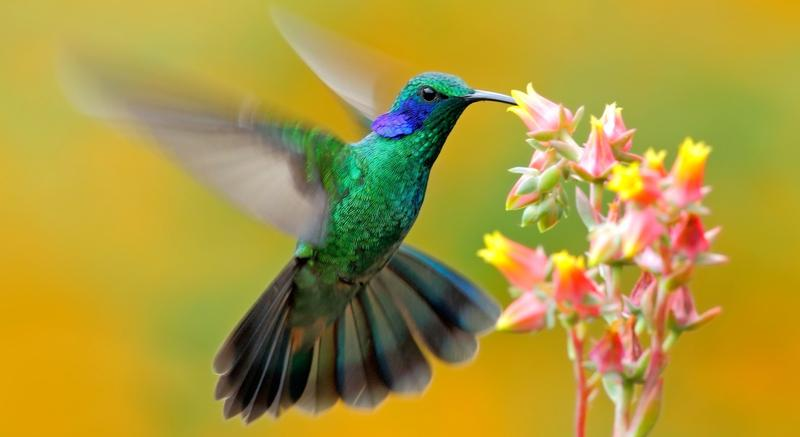
\includegraphics[width=4cm]{Hinh/chimruoi}}
\subsubsection{Dao động tuần hoàn}
\newghichu{Dao động tuần hoàn là dao động mà trạng thái chuyển động của vật được lặp lại như cũ sau những khoảng thời gian bằng nhau xác định (gọi là chu kì)}
\subsubsection{Dao động tự do}
\newghichu{\begin{itemize}
\item \textit{Dao động tự do} là dao động mà chu kì (tần số) chỉ phụ thuộc vào các đặc tính của hệ mà không phụ thuộc vào các yếu tố bên ngoài.
\item Dao động tự do xảy ra chỉ dưới tác dụng của nội lực.
\end{itemize}}
\subsubsection{Dao động điều hòa}
\newghichu{Dao động điều hòa là dao động trong đó li độ của vật là một hàm cos (hoặc sin) của thời gian}
%\setcounter{paragraph}{0}
\subsubsection{Phương trình dao động điều hòa}
\centerline{
\begin{tikzpicture}[draw=Mapcolor,very thick,>=stealth']
\foreach \x in {2,5}
{\draw [dashed] (\x,0)--++(-90:1.4); }
\draw (0,0)node[above]{$-A$}circle (1.5pt)--(10,0)node[above]{$A$}circle (1.5pt);
\draw (5,0)node[above]{ O}circle (1.5pt);
\draw[ball color=Mapcolor] (2,0) circle (.3);
\foreach \x in {0,10}
{\draw [dashed] (\x,0)--++(-90:1.8); }
\draw[<->] (0,-1.6)--node[midway,fill=white]{Chiều dài quỹ đạo L}++(0:10);
\draw[<->] (5,-1)--node[midway,fill=white]{Biên độ A}++(0:5);
\draw[<->] (2,-1)--node[midway,fill=white]{li độ x}++(0:3);
\draw[->,dashed] (2,0.5)--++(180:2)--++(90:0.3)--++(0:10)--++(90:0.3)--++(180:8);
\draw[decorate, decoration={brace, amplitude=5pt}] (10.2,1.3)--node[midway,right=3pt]{Chu kì T}++(-90:1);
\end{tikzpicture}
}
\centerline{\bth{\boder{x=A\cos(\omega t+\varphi)}}}
Trong đó:
\begin{itemize}
\item $x$ là li độ dao động, là khoảng cách từ gốc tọa độ (VTCB) đến vị trí của vật tại thời điểm $t$ đang xét: $-A \leq x \leq A$.
\item $A$ là biên độ dao động (luôn dương).
\item $\omega$ là tần số góc (luôn dương).
\item $\omega t+\varphi$ là pha của dao động tại thời điểm $t$.
\item $\varphi$ là pha ban đầu của dao động.
\end{itemize}
\begin{note}
\textit{Dao động điều hòa là trường hợp đơn giản nhất của dao động tuần hoàn}.
\end{note}
\subsubsection{Chu kì, tần số của dao động}
\begin{itemize}
\item \textbf{Chu kì T} của dao động điều hòa 
\begin{itemize}
\item là khoảng thời gian để vật thực hiện một dao động toàn phần. 
\item là khoảng thời gian \textit{ngắn nhất} để vật quay trở lại vị trí cũ, theo \textit{hướng cũ}.
\end{itemize}
\item \textbf{Tần số f} của dao động điều hòa là số dao động toàn phần thực hiện được trong một giây. 
\centerline{\bth{\boder{T=\dfrac{1}{f}=\dfrac{2\pi}{\omega}=\dfrac{\Delta t}{N}}\quad (s)
}}
Với $N$ là số dao động toàn phần vật thực hiện được trong thời gian $\Delta t$.

\end{itemize}
